\documentclass[11pt,a4paper]{article}

\usepackage[utf8]{inputenc}
\usepackage[T1]{fontenc}
\usepackage[polish]{babel}
\usepackage{graphicx}
\usepackage{booktabs}
\usepackage{float}
\usepackage{amsmath}
\usepackage[margin=2.3cm]{geometry}
\usepackage{enumitem}
\usepackage{xcolor}
\usepackage[hidelinks]{hyperref}

\title{\textbf{Biometria --- Projekt 3}\\[2mm]
\large Uwierzytelnianie twarzą \emph{in-the-wild}:\\
odporność na niską rozdzielczość (CCTV) oraz wiele twarzy na obrazie}
\author{}
\date{}

\begin{document}
\maketitle

%==================================================================
\section*{Dane autorów}
\begin{tabular}{ll}
Autorzy: & \emph{[Imię Nazwisko, nr indeksu]} \\
         & \emph{[Imię Nazwisko, nr indeksu]} \\
         & \emph{[Imię Nazwisko, nr indeksu]} \\
Termin laboratorium: & \emph{[dzień, godzina, grupa]} \\
\end{tabular}

%==================================================================
\section{Opis problemu}

Celem projektu jest system \textbf{uwierzytelniania na podstawie obrazu twarzy},
który zachowuje skuteczność na \emph{trudnych} próbkach pobieranych bez kontroli nad
otoczeniem (\emph{in-the-wild}). Zgodnie z poleceniem wybraliśmy dwa utrudnienia:

\begin{enumerate}[label=\textbf{\#\arabic*}]
\setcounter{enumi}{2}
\item[\textbf{\#3}] \textbf{Bardzo niska rozdzielczość / jakość} --- twarze wielkości
kilkudziesięciu pikseli, jak z kamer CCTV (scenariusz zbioru TinyFace).
\item[\textbf{\#1}] \textbf{Wiele twarzy na zdjęciu} --- na obrazie widocznych jest kilka
osób; system musi wybrać właściwą do uwierzytelnienia.
\end{enumerate}

Zgodnie z dopuszczeniem w poleceniu \textbf{korzystamy z gotowego, wstępnie wytrenowanego
modelu i \emph{nie} dotrenowujemy go}. Odporność na trudne dane budujemy wyłącznie
\emph{trikami na etapie wnioskowania} (ang. \emph{test-time}). Cel ilościowy: na próbkach
trudnych współczynnik FRR nie powinien wzrosnąć o więcej niż 5~punktów procentowych (pp),
a~True Identification Rate nie powinien spaść o więcej niż 5~pp względem próbek czystych,
przy minimalizacji FAR.

\paragraph{Wykorzystane źródła i narzędzia.}
\begin{itemize}[nosep]
\item \textbf{ArcFace} (Deng i in., 2019) --- funkcja straty i architektura sieci do
rozpoznawania twarzy; użyty backbone \texttt{iresnet50}, wagi \texttt{ms1mv3\_arcface\_r50}
(trenowane na zbiorze MS1MV3).
\item \textbf{InsightFace} (model detekcji \texttt{buffalo\_l}) --- detekcja twarzy i punktów
charakterystycznych oraz wyrównanie (\emph{alignment}).
\item Zbiory bazowe: \textbf{FaceCard} (LFW-podobny), zdjęcia własne członków grupy.
\item Scenariusz niskiej rozdzielczości inspirowany zbiorem \textbf{TinyFace}.
\end{itemize}

%==================================================================
\section{Metoda uwierzytelniania}

\subsection{Zasada działania}
Sieć ArcFace zamienia wyrównany obraz twarzy ($112\times112$~px) na
\textbf{embedding} --- wektor 512 liczb będący „odciskiem palca” twarzy. Embeddingi tej samej
osoby są do siebie zbliżone, różnych osób --- odległe. Podobieństwo mierzymy
\textbf{dystansem kosinusowym} $d = 1 - \cos(\theta)$ (mały dystans = ta sama osoba).
System działa w dwóch trybach:
\begin{itemize}[nosep]
\item \textbf{Weryfikacja (1:1)} --- porównanie próbki z galerią jednej deklarowanej osoby;
decyzja: akceptacja gdy $d \le$ próg.
\item \textbf{Identyfikacja (1:N)} --- porównanie z galeriami wszystkich wdrożonych osób
i wybór najbliższej (Top-1), z opcją odrzucenia (\emph{open-set}).
\end{itemize}

\subsection{Pipeline i modyfikacje uodparniające}
Każda próbka przechodzi przez łańcuch (rysunek koncepcyjny poniżej); pogrubione kroki to
nasze modyfikacje wprowadzone dla odporności:

\begin{center}
\fbox{\parbox{0.95\linewidth}{\centering
obraz $\rightarrow$ \textbf{detekcja odporna (padding)} $\rightarrow$ \textbf{selekcja
właściwej twarzy (\#1)} $\rightarrow$ ocena jakości \textbf{FIQA (\#3)} $\rightarrow$
\textbf{restauracja warunkowa (\#3)} $\rightarrow$ wyrównanie $112^2$ $\rightarrow$
embedding $+$ \textbf{TTA} $\rightarrow$ dopasowanie (galeria wielowzorcowa,
\textbf{próg adaptacyjny})
}}
\end{center}

\begin{description}[leftmargin=1.5em,style=nextline]
\item[Detekcja odporna na ciasne kadry (kluczowa modyfikacja).]
Zdjęcia FaceCard oraz kadry CCTV to \emph{ciasne wycięcia} --- twarz wypełnia cały obraz bez
marginesu, przez co detektor jej \emph{nie wykrywa}. Bez detekcji następuje awaryjne wycięcie
środka (\emph{center-crop}) \textbf{bez wyrównania}, co drastycznie psuje rozpoznawanie. Nasze
rozwiązanie: gdy detekcja na surowym obrazie zawiedzie, dokładamy margines (replikacja brzegu)
i~ponawiamy detekcję. To umożliwia poprawne wyrównanie. Modyfikacja podniosła skuteczność na
niskiej rozdzielczości z~$\sim$0\% do~$\sim$55\% (sama detekcja), a~z~pozostałymi trikami do~77\%.
\item[Selekcja właściwej twarzy (\#1).] Spośród wszystkich wykrytych twarzy wybieramy
kandydata na podstawie wielkości, centralności i pewności detekcji; przypadki niejednoznaczne
odrzucamy.
\item[Ocena jakości twarzy --- FIQA (\#3).] Liczbowa ocena jakości próbki (ostrość, rozmiar
twarzy), sterująca restauracją i progiem adaptacyjnym.
\item[Restauracja warunkowa (\#3).] Dla próbek o niskiej jakości stosujemy poprawę obrazu
przed rozpoznaniem.
\item[Test-Time Augmentation (TTA).] Embedding liczony dla kilku wariantów obrazu (m.in.
odbicie lustrzane) i uśredniany --- stabilniejszy wynik.
\item[Galeria wielowzorcowa.] Na osobę przechowujemy kilka embeddingów; próbkę porównujemy do
najbliższego z nich.
\item[Próg adaptacyjny.] Dla próbek o niskiej jakości próg decyzji jest delikatnie luzowany.
\end{description}

\subsection{Próg decyzji}
Próg dobieramy \textbf{automatycznie} na zbiorze czystym tak, aby FAR wynosił 1\%
(zgodnie z celem „minimalizować FAR”). Otrzymany próg operacyjny to dystans
$d^\star = 0{,}7735$, co odpowiada podobieństwu kosinusowemu $\cos\theta \approx 0{,}23$.
Próg adaptacyjny luzuje go do $\cos\theta \approx 0{,}15$ dla najgorszej jakości.

%==================================================================
\section{Zbiór danych, podział i subsampling}

\subsection{Źródła i podział na role}
Podział tożsamości jest \textbf{deterministyczny} (ziarno losowości $=42$, pełna
powtarzalność) i \textbf{rozłączny} --- żadna osoba nie występuje w dwóch rolach, co
zapobiega zawyżaniu wyników. Uwzględniamy tylko tożsamości mające $\ge 4$ zdjęcia.

\begin{table}[H]\centering
\begin{tabular}{lcl}
\toprule
Rola & Liczba osób & Zastosowanie (etap) \\
\midrule
\textbf{enrolled} (wdrożeni) & 100 & wzorce w bazie; \emph{w tym cała grupa} (etap wdrożenia) \\
\textbf{impostors} (impostorzy) & 120 & próbki „obcych” do odrzucenia (etap testu) \\
\textbf{distractors} (dystraktory) & 150 & dodatkowe twarze w scenach \#1 (generacja danych) \\
\bottomrule
\end{tabular}
\caption{Podział tożsamości na role. Osoby wdrożone i impostorzy są rozłączni.}
\end{table}

\subsection{Procedura wdrożenia (enrollment)}
Dla każdej z 100 wdrożonych osób bierzemy \textbf{3 pierwsze czyste zdjęcia} i zapisujemy
\textbf{3 osobne embeddingi} (galeria wielowzorcowa --- nie uśredniamy). Zdjęcia użyte do
wdrożenia są wykluczone z testu.

\subsection{Tworzenie zbiorów testowych}
Wszystkie próbki trudne powstają z \emph{czystych} zdjęć osób wdrożonych, dzięki czemu mamy
\textbf{pary} czyste$\leftrightarrow$trudne tej samej osoby i możemy mierzyć degradację wprost.

\begin{description}[leftmargin=1.5em,style=nextline]
\item[Zbiór czysty (clean) --- 1103 próbki.] 983 próbki \emph{genuine} (zdjęcia osób
wdrożonych nieużyte do wdrożenia, do 10 na osobę) $+$ 120 próbek \emph{impostor} (po 1
zdjęciu każdej osoby niewdrożonej). Punkt odniesienia.
\item[Zbiór trudny \#3 (lowres) --- 2949 próbek.] Z każdego czystego zdjęcia genuine
generujemy 3 warianty degradacji CCTV: zmniejszenie twarzy do \textbf{20--40~px}, opcjonalne
rozmycie i szum, kompresja JPEG (jakość 35--65), powiększenie z powrotem do $112$~px.
\item[Zbiór trudny \#1 (multiface) --- 2949 próbek.] Z każdego czystego zdjęcia genuine
budujemy scenę $512\times512$~px zawierającą twarz właściwej osoby oraz \textbf{1--3 twarze
dystraktorów}.
\end{description}

\begin{table}[H]\centering
\begin{tabular}{lcccc}
\toprule
Zbiór & Próbki & w tym genuine & w tym impostor & Etap \\
\midrule
clean      & 1103 & 983  & 120 & odniesienie \\
lowres (\#3) & 2949 & 2949 & --- & test trudny \\
multiface (\#1) & 2949 & 2949 & --- & test trudny \\
\midrule
\textbf{razem} & \textbf{7001} & & & \\
\bottomrule
\end{tabular}
\caption{Liczności zbiorów. Trudnych łącznie 5898 (wymóg $\ge$5000, zbalansowane $\approx$50/50);
czystych 1103 (wymóg $\ge$1000).}
\end{table}

\begin{figure}[H]\centering
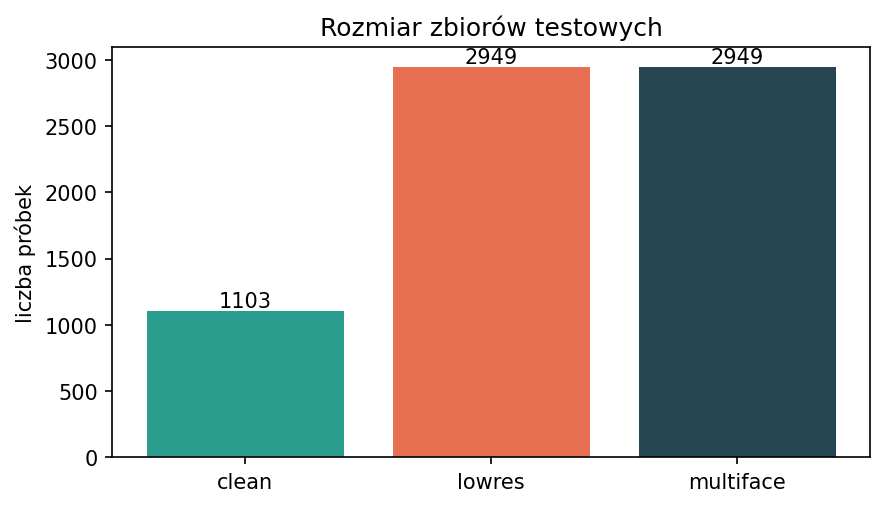
\includegraphics[width=0.55\linewidth]{img/dataset_sizes.png}
\hfill
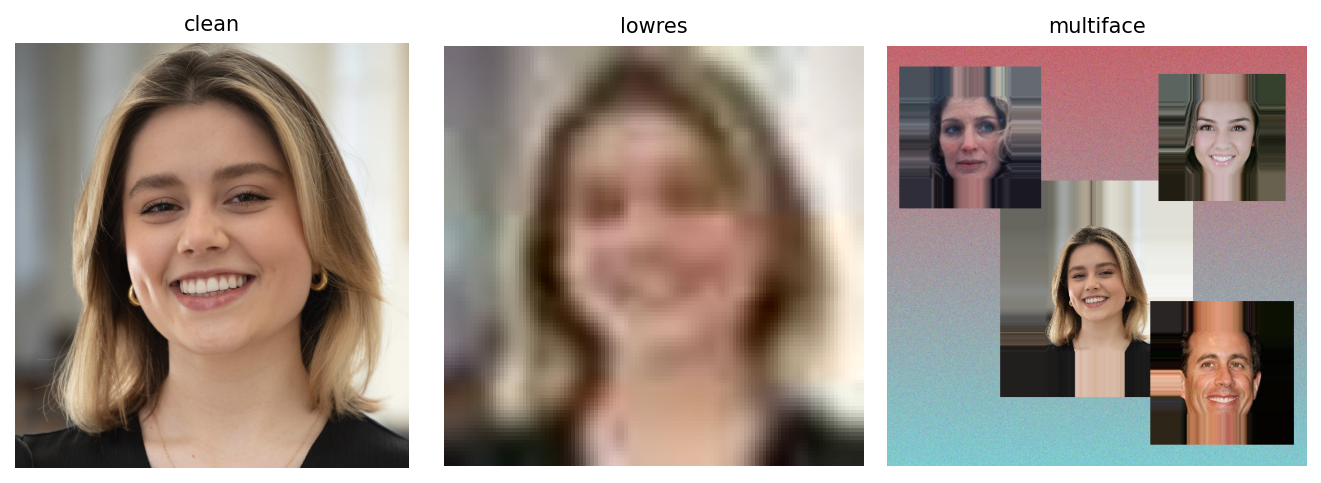
\includegraphics[width=0.42\linewidth]{img/examples.png}
\caption{Po lewej: rozmiary zbiorów testowych. Po prawej: ta sama osoba w wariancie czystym,
niskiej rozdzielczości (\#3) i wielu twarzy (\#1).}
\end{figure}

%==================================================================
\section{Procedura uwierzytelniania i testowania}

\subsection{Uwierzytelnianie}
Próbka przechodzi przez opisany pipeline, otrzymujemy jej embedding, liczymy dystans
kosinusowy do galerii i podejmujemy decyzję (weryfikacja: $d\le$ próg; identyfikacja:
najbliższa galeria, z opcją odrzucenia). Przetwarzanie jednej próbki trwa ułamek sekundy
(wymóg $<30$~s spełniony).

\subsection{Metryki}
\begin{itemize}[nosep]
\item \textbf{FRR} (False Rejection Rate) --- odsetek osób prawdziwych błędnie odrzuconych.
\item \textbf{FAR} (False Acceptance Rate) --- odsetek impostorów błędnie zaakceptowanych.
\item \textbf{TIR} (True Identification Rate) --- odsetek poprawnych identyfikacji Top-1
(oraz Top-5).
\item \textbf{EER} (Equal Error Rate) --- punkt, w którym FAR${=}$FRR (im mniej, tym lepiej).
\end{itemize}

\subsection{Prace nad korektą wyników na próbkach zaburzonych}
W~trakcie ewaluacji zidentyfikowaliśmy i naprawiliśmy dwa kluczowe problemy:
\begin{enumerate}[nosep]
\item \textbf{Brak wyrównania na ciasnych kadrach} --- detekcja zawodziła na 100\% próbek
lowres; wprowadzenie \emph{detekcji odpornej z paddingiem} podniosło TIR z 0\% do $\sim$77\%.
\item \textbf{Niestabilny dobór progu} --- pierwotny próg z punktu EER na zbiorze idealnie
rozdzielonym był nieokreślony; zastąpiliśmy go progiem przy zadanym FAR${=}$1\%.
\end{enumerate}

%==================================================================
\section{Wyniki}

\begin{table}[H]\centering
\begin{tabular}{lrrrrr}
\toprule
Utrudnienie & EER & FRR & FAR & TIR@1 & TIR@5 \\
\midrule
clean            & 0{,}57\% & 0{,}41\%  & 1{,}24\% & 99{,}59\% & 99{,}79\% \\
\#1 multiface    & 0{,}59\% & 0{,}44\%  & 1{,}22\% & \textbf{99{,}56\%} & 99{,}66\% \\
\#3 lowres       & 10{,}62\% & 17{,}24\% & 2{,}62\% & \textbf{77{,}37\%} & 87{,}48\% \\
\bottomrule
\end{tabular}
\caption{Wyniki pełnego systemu (próg $d^\star=0{,}7735$, AUC na clean $=0{,}999$).}
\end{table}

\begin{table}[H]\centering
\begin{tabular}{lrrc}
\toprule
Utrudnienie & $\Delta$FRR & $\Delta$TIR@1 & Cel $\le$5~pp \\
\midrule
\#1 multiface & $+0{,}03$~pp & $-0{,}03$~pp & \textcolor{green!50!black}{\textbf{spełniony}} \\
\#3 lowres    & $+16{,}83$~pp & $-22{,}21$~pp & \textcolor{red}{\textbf{niespełniony}} \\
\bottomrule
\end{tabular}
\caption{Degradacja względem zbioru czystego. Multiface mieści się w celu; lowres przekracza
go o~$\sim$17~pp (TIR) / $\sim$12~pp (FRR).}
\end{table}

\begin{figure}[H]\centering
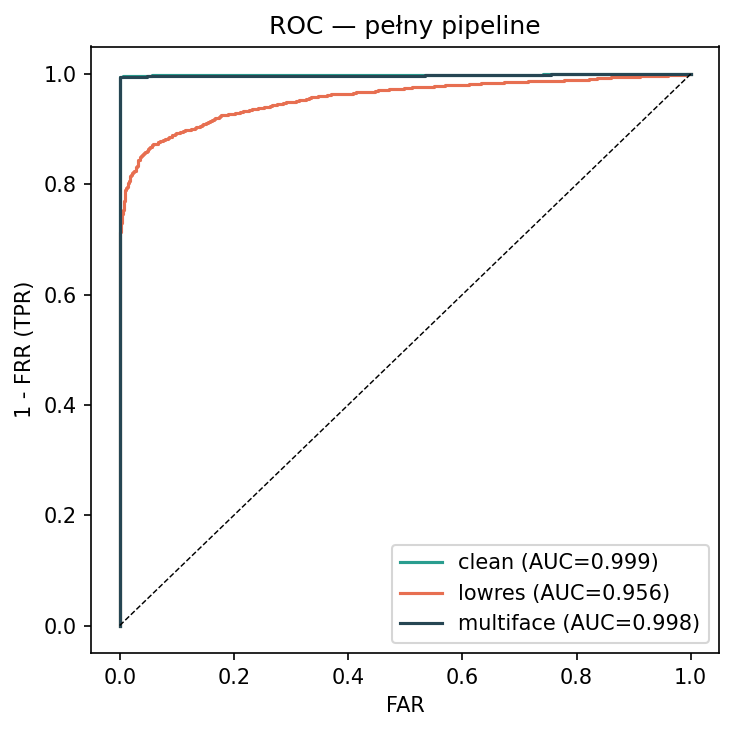
\includegraphics[width=0.42\linewidth]{img/roc.png}\hfill
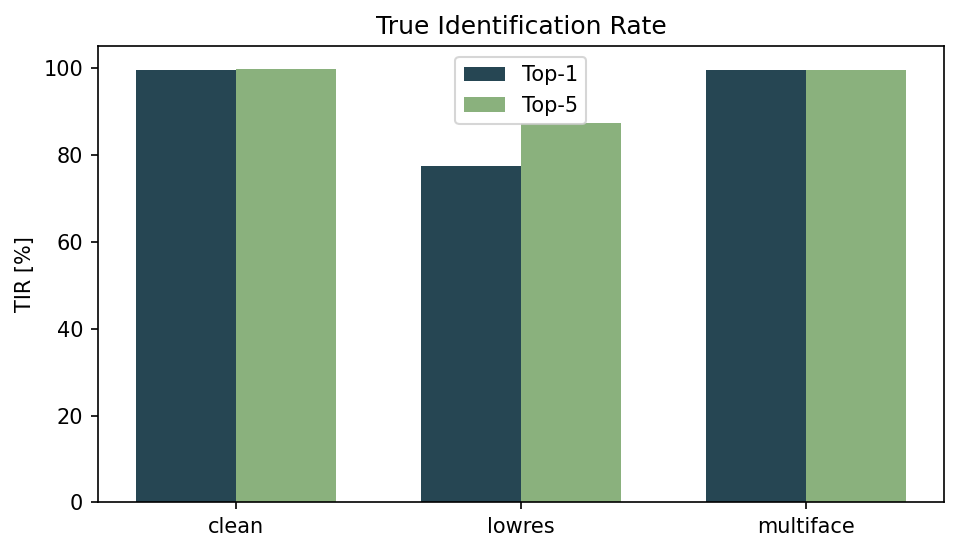
\includegraphics[width=0.55\linewidth]{img/tir.png}
\caption{Po lewej: krzywe ROC (weryfikacja). Po prawej: True Identification Rate.}
\end{figure}

\begin{figure}[H]\centering
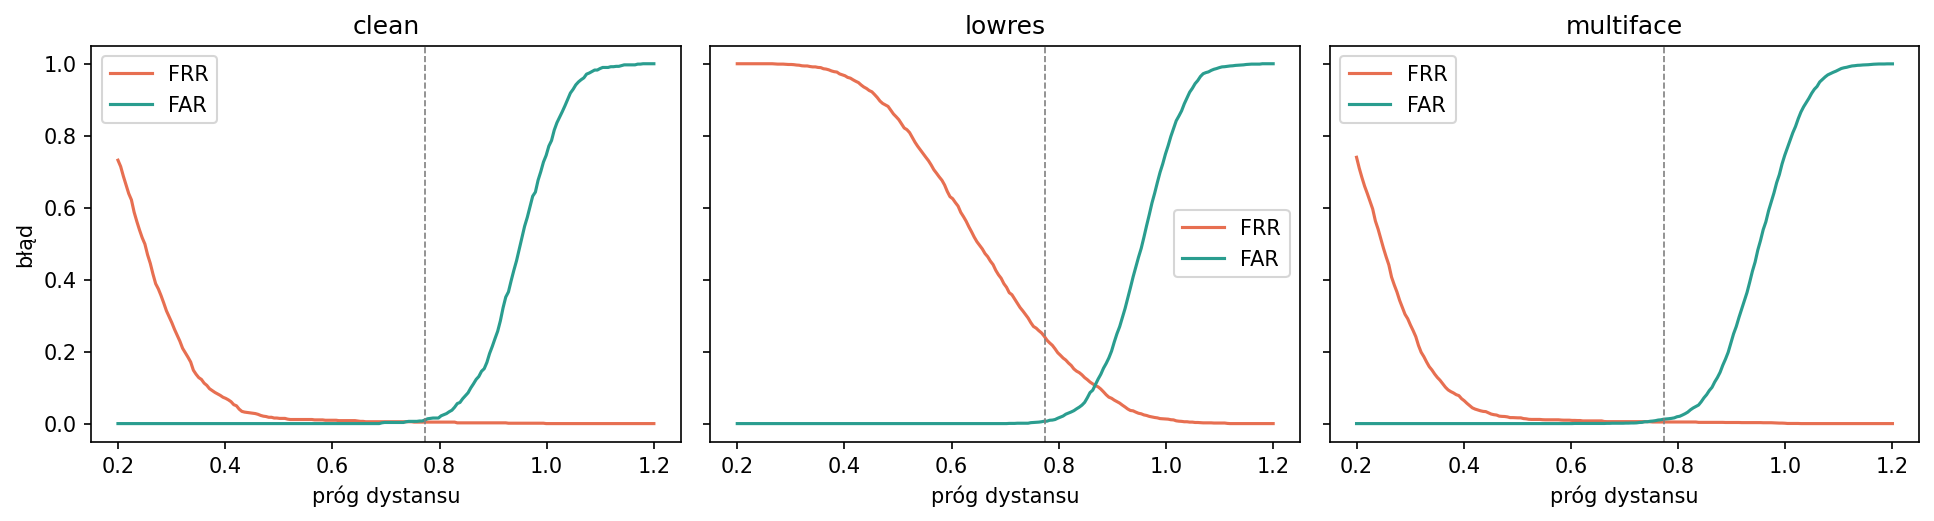
\includegraphics[width=\linewidth]{img/far_frr.png}
\caption{FAR i FRR w funkcji progu dla każdego utrudnienia (linia przerywana --- próg
operacyjny). Dla lowres rozkłady genuine i impostor zachodzą na siebie, stąd kompromis.}
\end{figure}

\begin{figure}[H]\centering
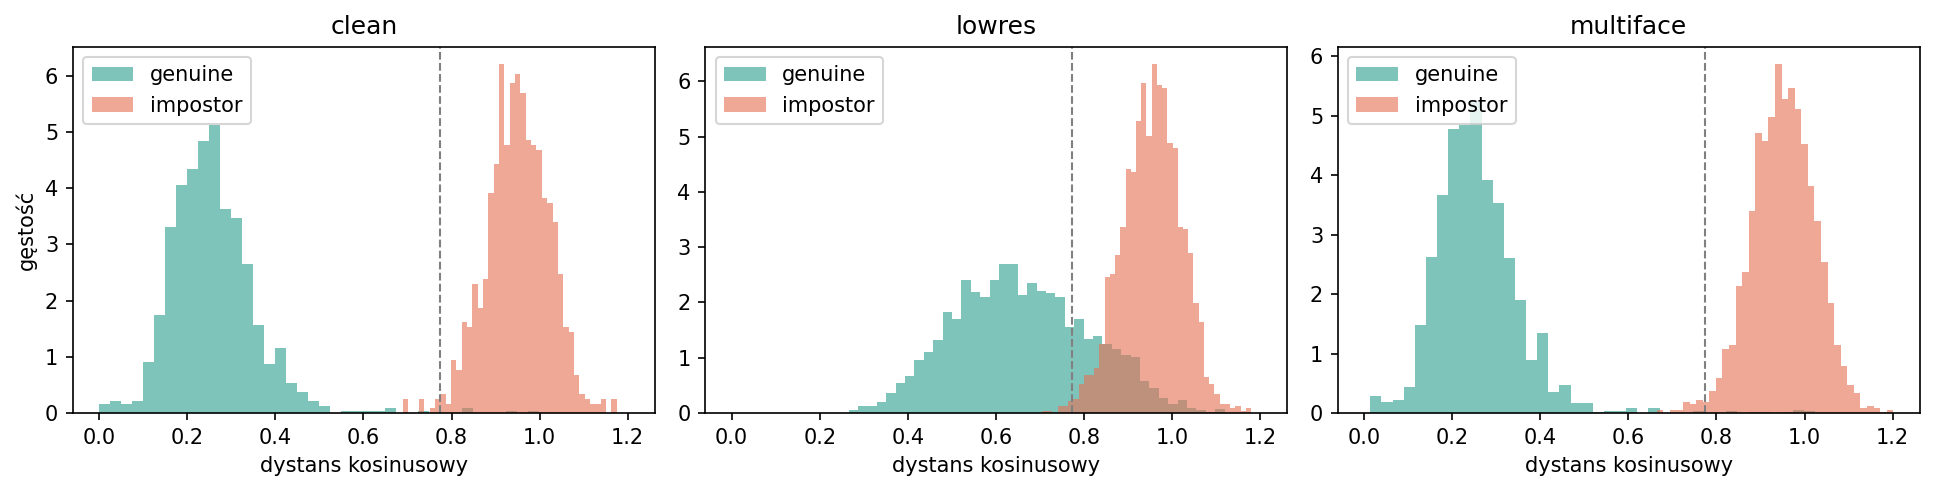
\includegraphics[width=\linewidth]{img/distances.png}
\caption{Rozkłady dystansów genuine (zielony) vs impostor (czerwony). Dla clean i multiface
istnieje wyraźna przerwa; dla lowres rozkłady się nakładają --- to obrazuje twardy limit
rozpoznawania twarzy niskiej rozdzielczości.}
\end{figure}

\subsection{Ablacja --- wkład trików}
Porównujemy pełny system z wariantem bazowym (bez selekcji, restauracji, TTA i progu
adaptacyjnego).

\begin{table}[H]\centering
\begin{tabular}{lrrrr}
\toprule
Utrudnienie & TIR@1 \emph{bazowy} & TIR@1 \emph{pełny} & FRR \emph{bazowy} & FRR \emph{pełny} \\
\midrule
clean         & 99{,}59\% & 99{,}59\% & 0{,}51\% & 0{,}41\% \\
\#1 multiface & 14{,}72\% & \textbf{99{,}56\%} & 85{,}42\% & 0{,}44\% \\
\#3 lowres    & 55{,}68\% & \textbf{77{,}37\%} & 45{,}30\% & 17{,}24\% \\
\bottomrule
\end{tabular}
\caption{Ablacja. Dla \#1 całą skuteczność daje \emph{selekcja twarzy} (14{,}7\%$\to$99{,}6\%);
dla \#3 restauracja $+$ TTA dokładają $+$21{,}7~pp.}
\end{table}

\begin{figure}[H]\centering
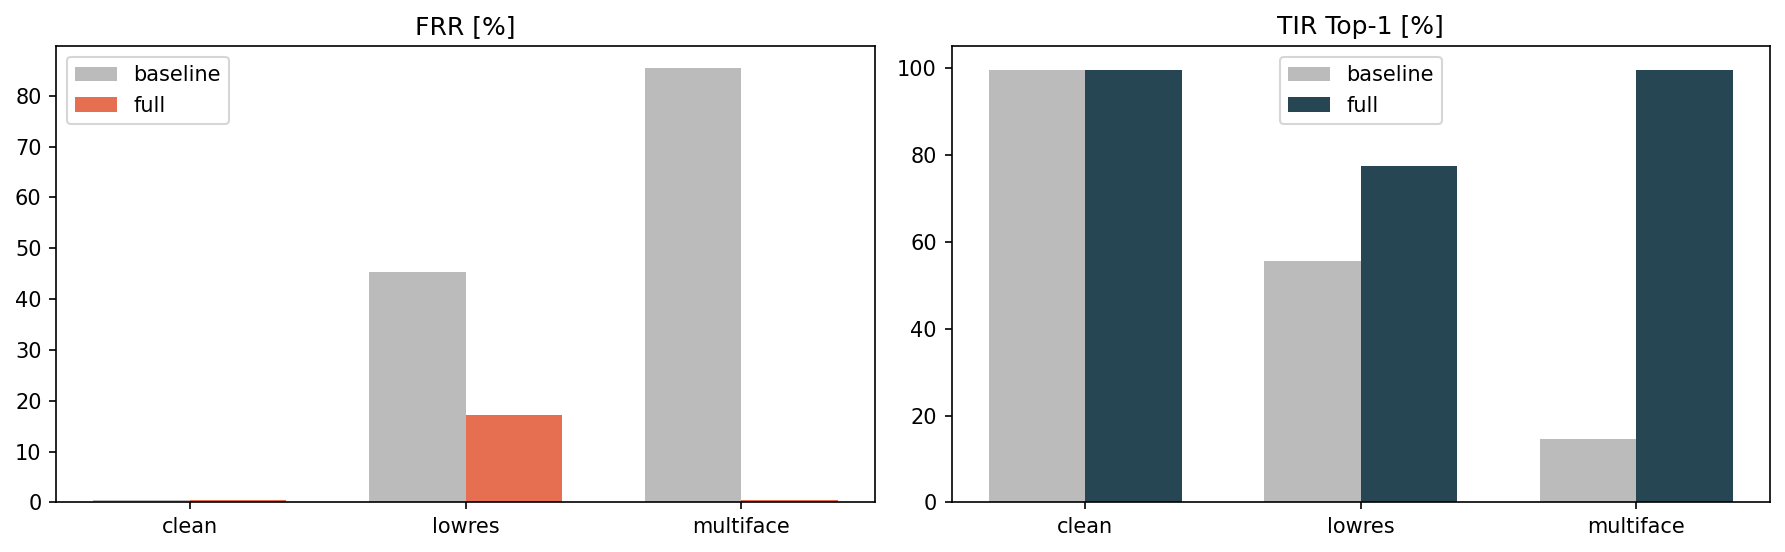
\includegraphics[width=\linewidth]{img/ablation.png}
\caption{Ablacja: wariant bazowy vs pełny system (FRR i TIR Top-1).}
\end{figure}

\subsection{Porównanie z modelem bazowym i literaturą}
Na próbkach \textbf{czystych} (wysoka rozdzielczość) nasz system osiąga TIR@1 $=99{,}6\%$ ---
zgodnie z poziomem raportowanym przez autorów ArcFace dla danych frontalnych dobrej jakości
($\sim$99{,}8\% na LFW). Potwierdza to, że pipeline nie wprowadza degradacji w warunkach
nominalnych.

Dla \textbf{niskiej rozdzielczości} nasz wynik 77\% rank-1 (na syntetycznej degradacji
20--40~px) jest na poziomie lub powyżej typowych wyników gotowych modeli rozpoznawania twarzy
raportowanych na zbiorze TinyFace (rząd $\sim$30--60\% rank-1 dla modeli „z półki”, $\sim$60--70\%
dla metod dedykowanych niskiej rozdzielczości). \emph{Uwaga:} porównanie jest poglądowe ---
nasza degradacja jest syntetyczna i protokół nie jest identyczny z TinyFace, więc liczb nie
należy zestawiać wprost.

%==================================================================
\section{Wnioski}

\begin{itemize}[leftmargin=1.5em]
\item \textbf{Utrudnienie \#1 (wiele twarzy) --- cel w pełni osiągnięty} ($\Delta$TIR
$=-0{,}03$~pp). Ablacja pokazuje, że decydująca jest \emph{selekcja właściwej twarzy}: bez niej
system wybiera przypadkową twarz i skuteczność spada do 14{,}7\%. Problem ma więc charakter
„logiczny” (wybór celu), a~nie utraty informacji, i daje się rozwiązać trikiem test-time.

\item \textbf{Utrudnienie \#3 (niska rozdzielczość) --- cel niespełniony} ($\Delta$TIR
$=-22{,}2$~pp, $\Delta$FRR $=+16{,}8$~pp). Mimo to triki dały duży zysk: od $\sim$0\% (bez
wyrównania) przez 55\% (sama detekcja odporna) do 77\% (pełny system). Pozostała luka to
\textbf{twardy limit} --- przy twarzy 20--40~px sieć fizycznie traci część informacji o
tożsamości, czego nie odzyska się bez dotrenowania modelu lub ciężkiej restauracji
generatywnej (np. GFPGAN/CodeFormer).

\item \textbf{Najważniejsza modyfikacja} to detekcja odporna na ciasne kadry --- pojedyncza
zmiana decydująca o sensowności wyników na obu utrudnieniach.

\item \textbf{Kierunki dalsze:} (i) generatywna restauracja twarzy dla lowres; (ii)
dotrenowanie/„low-resolution aware” fine-tuning backbone; (iii) krzywa TIR vs rozdzielczość
twarzy w celu wyznaczenia progu, od którego cel $\le$5~pp jest osiągany.
\end{itemize}

\end{document}
